%%%%%%%%%%%%%%%%%%%%%%
\subsection{Example: Cu metal at 3 temperature}
\begin{frame}[fragile] \frametitle{Example: Cu metal at 3 temperature}

\begin{cenpage}{130mm}
    A very simple example of a Multi-Data-Set Fit:

    Cu metal, at 3 different  temperatures: 10K, 50K 150K.

   \begin{columns}
     \begin{column}{55mm}
        \vmm  Path Parameters:
       \begin{itemize}
       \item $E_0$:  Same for all $T$
       \item $S_0^2$  Same for all $T$
       \item $R$:  expands linearly with $T$ (slope + offset).
       \item $\sigma^2$:  goes as Einstein temperature (as before).
       \end{itemize}

       {\RedEmph{12 parameters become 5.}}

       \vmm Fit range: \vmm

       \hspace{2mm} $R = [1.60, 2.75] \rm\, \AA$

       \vmm
       \hspace{2mm}  $k = [1.50, 18.50] \rm\, \AA^{-1}$
     \end{column}
     \begin{column}{65mm}

  \begin{CodeBlock}{60mm}{Cu at three temperatures}

# define fitting parameter group
pars = group(amp      = param(1, vary=True),
             del_e0   = guess(2.0),
             theta    = param(250, min=10, vary=True),
             dr_off   = guess(0),
             dr_slope = guess(0) )

# define 3 Feff Path, give expressions for Path Parameters
path1_10  = feffpath('feff0001.dat',
                     s02='amp', e0='del_e0',
                     deltar='dr_off + 10*dr_slope',
                     sigma2='sigma2_eins(10, theta)')

path1_50  = feffpath('feff0001.dat',
                     s02='amp', e0='del_e0',
                     deltar='dr_off + 50*dr_slope',
                     sigma2='sigma2_eins(50, theta)')

path1_150 = feffpath('feff0001.dat',
                     s02='amp', e0='del_e0',
                     deltar='dr_off + 150*dr_slope',
                     sigma2='sigma2_eins(150, theta)')

   \end{CodeBlock}
 \end{column}
\end{columns}
\end{cenpage}
\end{frame}


%%%%%%%%%%%%%%%%%%%%%%
\subsection{Example: Cu metal Results}
\begin{frame}[fragile] \frametitle{Example: Cu metal Results}

  \begin{cenpage}{135mm}

  \begin{tabular}{ll}
    \begin{minipage}{60mm}
      \begin{tabular}{lll}
        {\ } &{\tt{amp}}  &   $0.91(0.08)$ \\
        &{\tt{theta}}  &   $233.5(19.6) \rm\, K $ \\
        &{\tt{del\_e0}}  &   $0.4(1.3) \rm \, eV$ \\
        & {\tt{dr\_off}} &   $0.002(0.003) \rm \, {\AA}/K $ \\
        &{\tt{dr\_slope}}   &    $0.5(1.8)\times 10^{-5} \rm \, {\AA}$ \\
      \end{tabular}
  \vmm
\end{minipage} &
\begin{minipage}{60mm}
  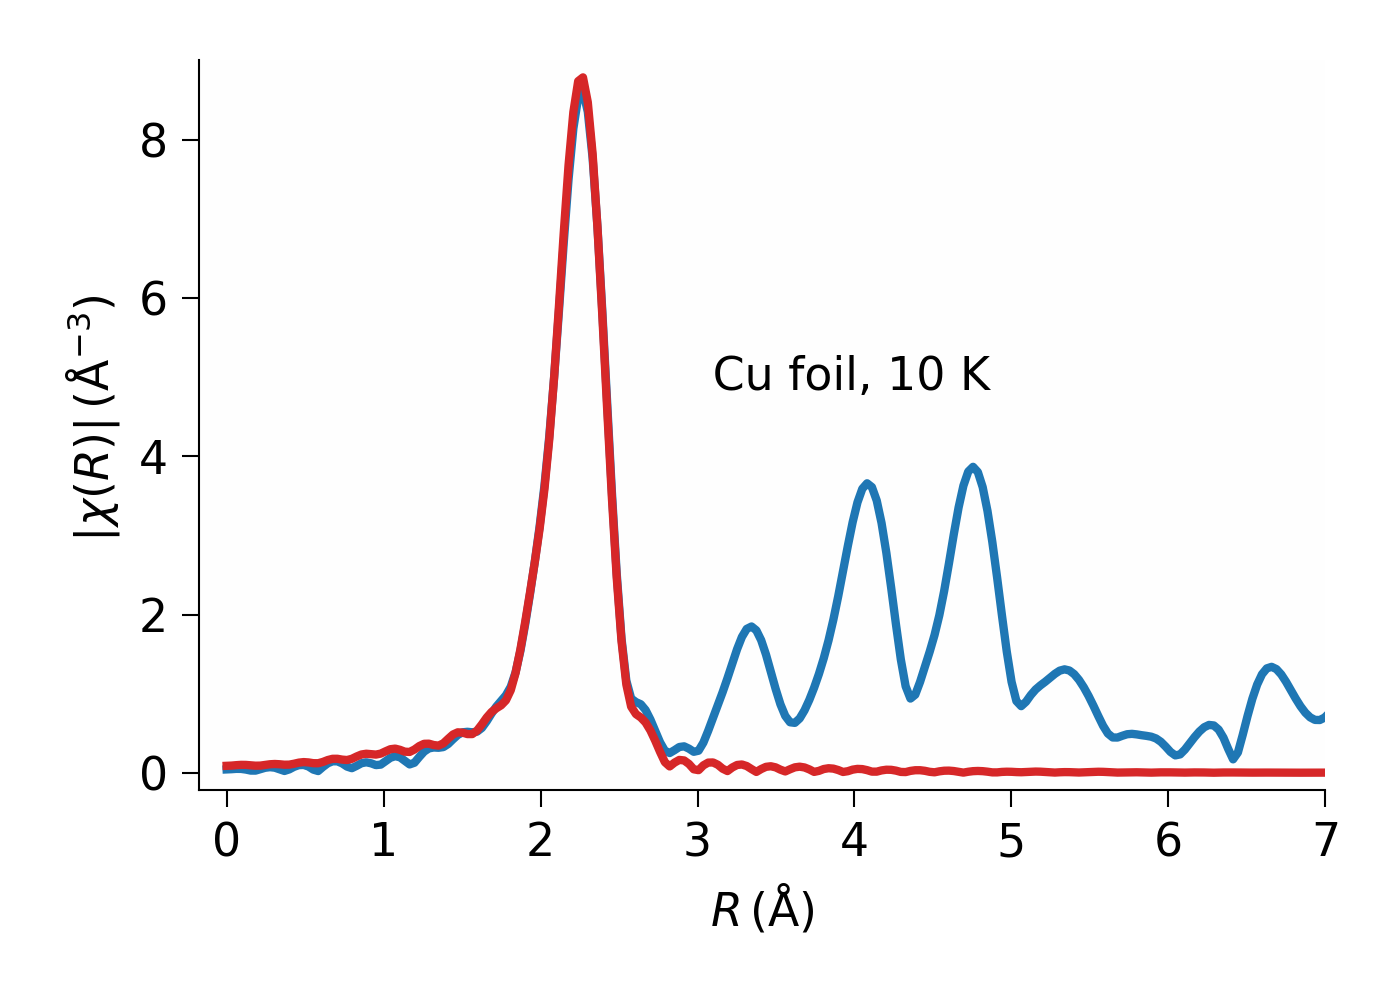
\includegraphics[width=56mm]{figs/Cu3temp/cu3temp_mag10}
\end{minipage} \\
\begin{minipage}{60mm}
  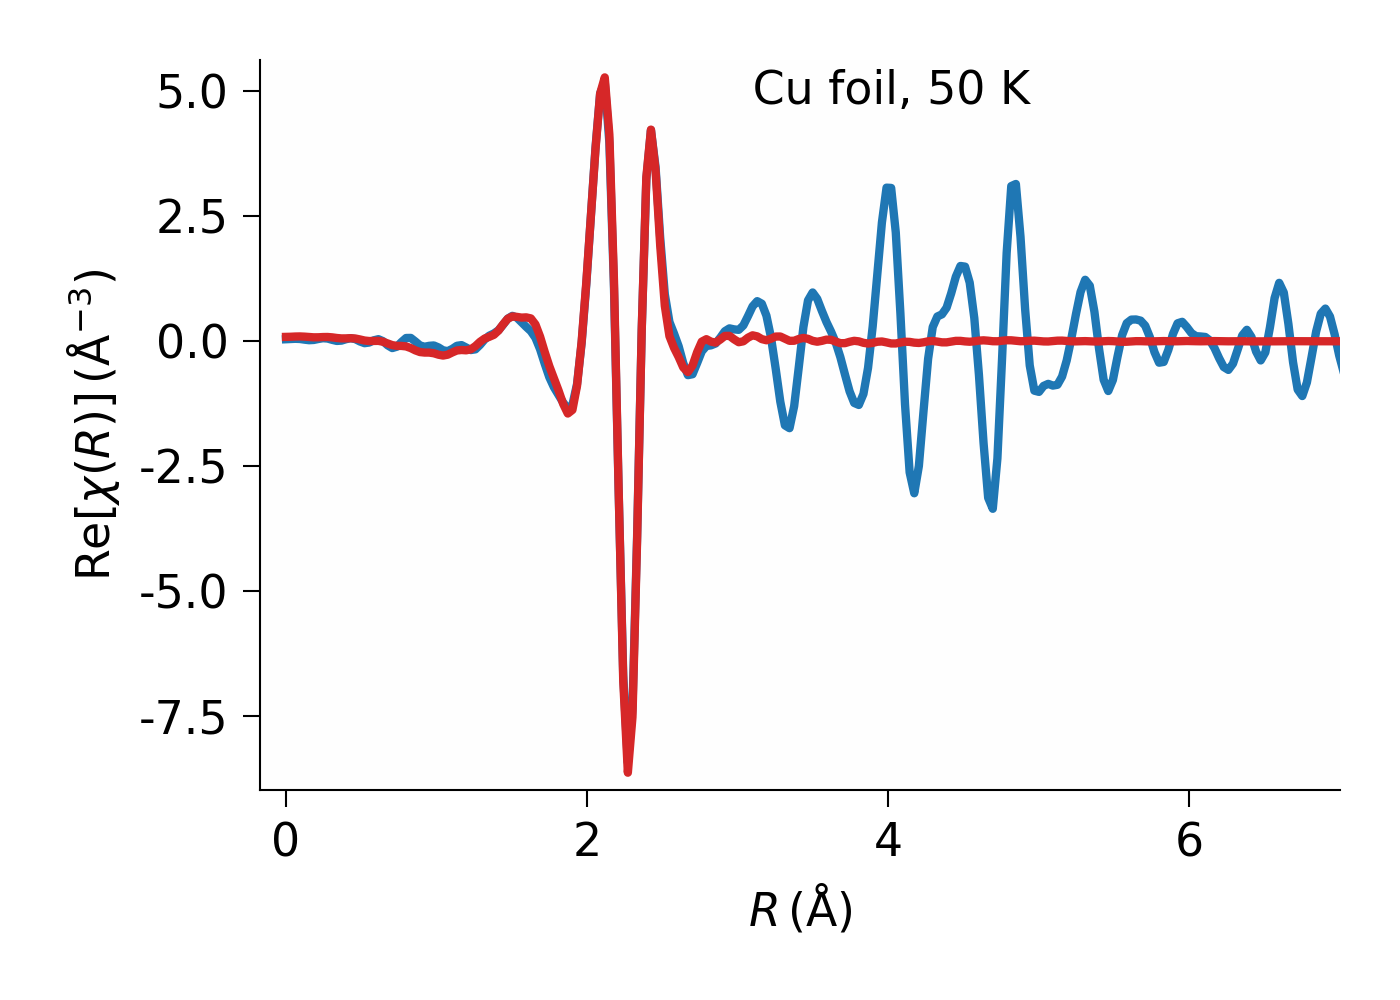
\includegraphics[width=56mm]{figs/Cu3temp/cu3temp_re50}
\end{minipage} &
\begin{minipage}{60mm}
  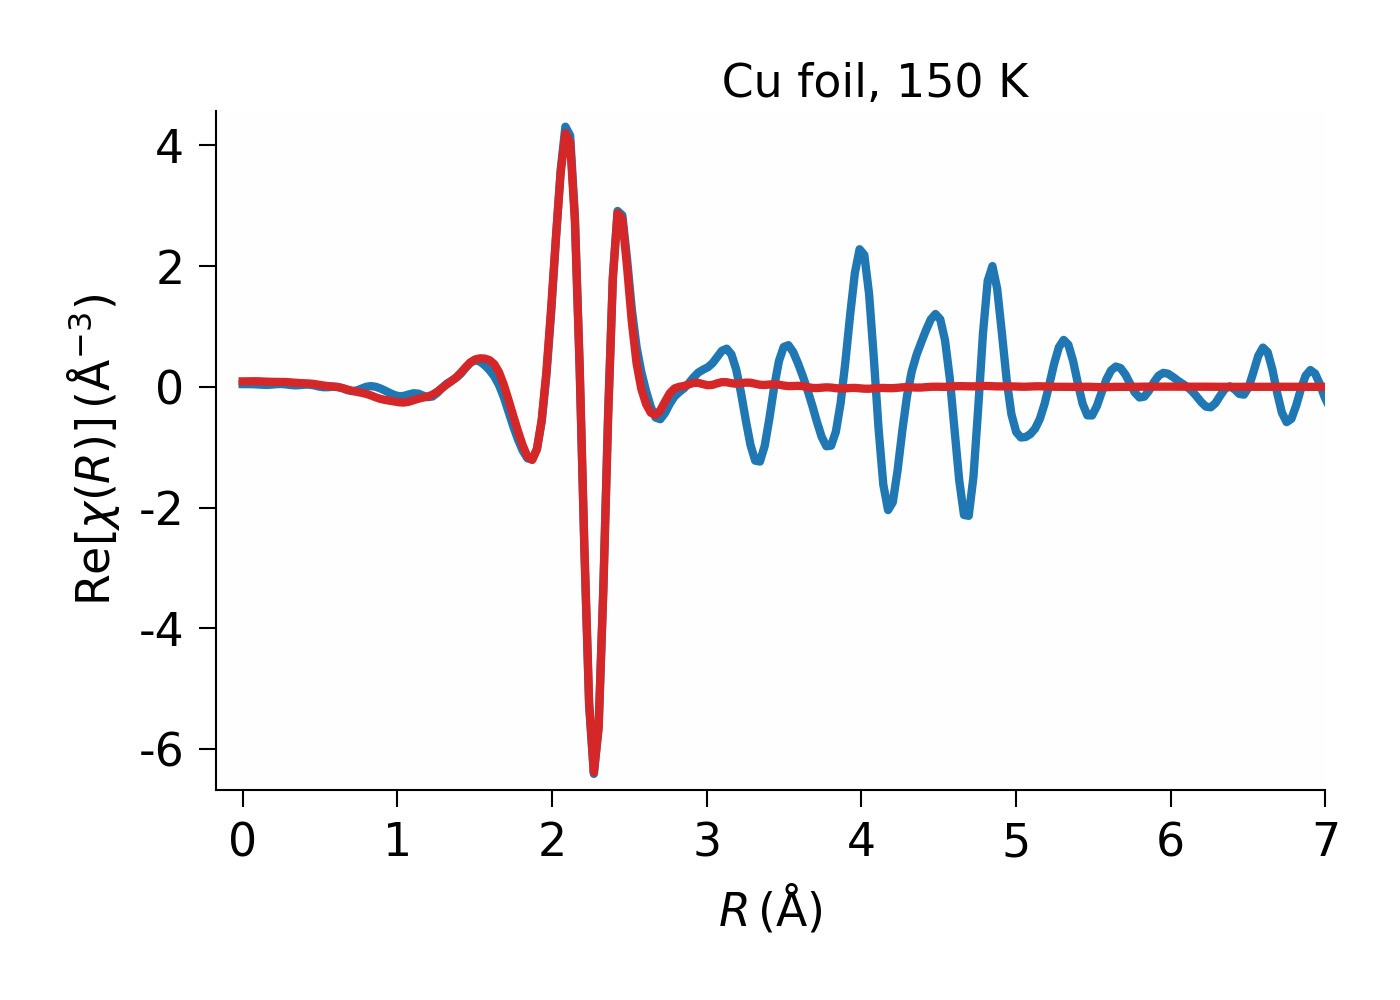
\includegraphics[width=56mm]{figs/Cu3temp/cu3temp_re150}
\end{minipage}\\
  \end{tabular}
\end{cenpage}

\end{frame}

%%%%%%%%%%%%%%%%%%%%%%
% \begin{slide}{Room Temperature Cu Fit }

%   Simple fit to first shell of Cu foil (300K): $k = [2,16] \rm\,
%     \AA^{-1}$, $R = [1.7,2.6] \rm\, \AA$, $k$-weight=2, $N_{\rm idp} = 8.4
%     $.  Fit results and statistics:


%     {
%       \hspace{0.1mm}\begin{tabular}{lll}
%         $R = 2.548(0.007) \, \rm\AA$
%         &
%         $\Delta E_0 = 4.5(0.6)$
%         &
%         $C_3      = 9(9) \times10^{-5} \rm\, \AA^3$
%         \\
%         $\epsilon_k = 1.6 \times 10^{-4}$
%         &
%         $S_0^2 = 0.96(0.04)$
%         &
%         $\sigma^2 = 8.5(0.3) \times10^{-3} \rm\, \AA^2$
%         \\
%         $\chi^2 = 678$ &
%         $\chi^2_\nu = 196.7$   & ${\cal{R}} = 0.00107 $\\
%       \end{tabular}
%     }

%     \vmm
%       \begin{tabular}{lcl}
%         \wgraph{49mm}{errors/cufit02} & \hspace{2mm} &
%         \wgraph{49mm}{errors/cufit01} \\
%       \end{tabular}

%       \begin{itemize}
%       \item ${\cal{R}} = 0.1\% $ -- a good fit!  But like $\chi^2_\nu$,
%         ${\cal{R}}$ is larger than the $\epsilon_k$ suggests.
%       \item These error bars account for correlations.  They increase
%         $\chi^2$ by $\chi^2_\nu$ (not 1), which scales them by
%         $\sqrt{\chi^2_\nu}\approx 14$ over ``increase $\chi^2$ by 1''.
%       \end{itemize}

%       \vmm
% \vfill
% \end{slide}
